\documentclass{beamer}


\usepackage[spanish]{babel}
\usepackage[T1]{fontenc}
\usepackage[utf8]{inputenc}

\usepackage{graphics}

\usepackage{fancyvrb} %fancy verbatim
\usepackage{color}

\graphicspath{{img/}}

\usetheme{Madrid}
\usecolortheme{beaver}
\setbeamercovered{transparent}

% \usepackage{beamerthemesplit} // Activate for custom appearance


\title{Modelación Basada en Agentes}
\author{Dr. Felipe Contreras}
\date{\today}

\begin{document}

\frame{\titlepage}

\section[Outline]{}
\frame{\tableofcontents}

\section{Antecedentes}

\subsection{Sistemas Complejos}
\frame{\alert{Sistemas Complejos}}
  \setbeamercovered{transparent}
\begin{frame}[t]
  \frametitle{Características}
  \begin{itemize}[<+-| alert@+>]
  \item Sistema: Conjunto de elementos o partes conectadas entre sí, que llevan acabo cierta función
  \item Complejo $\neq$ Complicado
  \item Presentan auto-organización
  \item Exhiben propiedades emergentes (``el todo es más que la suma de sus partes'')
  \begin{enumerate}[<+-| alert@+>]
  \item Muchos elementos
  \item Las interacciones son dinámicas
  \item Elementos influyen y son influidos por los demás
  \item Las interacciones son no lineales (pequeñas ``causas'', pueden tener ``efectos'' grandes)
  \item Las interacciones son recursivas
  \item Son abiertos % interacturan con otros sistemas
  \item Operan lejos del equilibrio
  \item Tienen una historia
  \item Los elementos actúan con información local
  \end{enumerate}
  \end{itemize}
  \end{frame}

\subsection{Mapeos Discretos}
\frame{\alert{Mapeos Discretos}}
\frame{
  \frametitle{Mapeos discretos}
  \begin{itemize}[<+->]
  \item $y = f(x)$
  \item $x_{1} = f(x_{0})$
  \item $x_{2} = f(x_{1}), x_{3}=f(x_{2}), x_{4} = f(x_{3}), ...$
  \end{itemize}
}
\frame{\frametitle{Representación gráfica}
\begin{block}{}
\begin{center}
\includegraphics<+>[height=.5\textheight]{mapeo1}
\includegraphics<+>[height=.5\textheight]{mapeo2}
\only<3>{ Programa ``logistica''}
\includegraphics<+>[width=.8\textwidth]{mapeo3}
\end{center}
\end{block}
}
\frame
{
  \frametitle{Características}

  \begin{itemize}[<+->]
  \item Converge (a un punto)
  \item No converge: tiene ciclo límite
  \item No converge: órbita densa
  \end{itemize}
}

\subsection{Autómatas Celulares}
\frame{\alert{Autómatas Celulares}}

\begin{frame}[t]
  \frametitle{Definición (genérica)}
  \begin{itemize}[<+->]
  \item Un AC consiste de autómatas (llamados también celdas o sitios) idénticos, dispuestos uniformemente en los puntos de una látice $D$-dimensional de un espacio discreto. Normalmente D=$1, 2,$ o $3$
  \item Cada autómata es una variable dinámica y su cambio temporal esta dado por la expresión:
  $$s_{t+1}(x) = F (s_{t}(x + x_{0}), s_{t}(x + x_{1}),\ldots , s_{t}(x + x_{n-1}))$$
  \item $s_{t}(x)$ es el estado de un autómata localizado en $x$ en el tiempo $t$
  \item $F$ es la función de transición de estado
  \item y $N=\{x_{0}, x_{1}, \ldots, x_{n-1}\}$ es la \textit{vecindad}
  \item por lo general se aplica la misma $F$ y la misma vecindad uniformemente a todas las posiciones espaciales
  \end{itemize}
\end{frame}

\begin{frame}[t]
  \frametitle{Definición (genérica)}
  \begin{itemize}[<+->]
  \item Fueron inicialmente desarrolladas por John von Newmann y su colaborador Stanislaw Ulam 
  \item Constituyen una forma de describir dinámicas espacio-temporales altamente no lineales de una manera simple y concisa
  \item Se utilizan para diversos campos como la dinámica molecular, hidrodinámica, propiedades físicas de materiales, procesos químicos de reacción-difusión, crecimiento y morfogénesis de organismos vivos, etc. [Sayama p.185 y ss]
  \end{itemize}
\end{frame}

\begin{frame}[t]
  \frametitle{AC 1D: Definición práctica}
  \begin{columns}[t]
  \column{.5\textwidth}
  \begin{block}{}
	\begin{itemize}[<+->]
		\item Vocabulario $\sigma$ de $n$ símbolos
		\item Organización de $m$ de estos símbolos en un estado inicial $E_{0}$
		\item Tamaño de vecindad o radio $\rho$
		\item Condiciones en la frontera (cíclica, terminación, valor único)
		\item Regla de evolución (función de mapeo)
	\end{itemize}
  \end{block}
   \column{.5\textwidth}
  \begin{center}
	\only<1> {$\sigma = \{0, 1\}$, $n=2$}
	\includegraphics<2>[width=.9\textwidth]{automata1}
	\only<3> {$\rho=3$}
	\includegraphics<4>[width=.9\textwidth]{automata2}
	\includegraphics<5>[height=.4\textheight]{automata3}
  \end{center}
  \end{columns}
\end{frame}

\begin{frame}[t]
  \frametitle{Regla de evolución}
  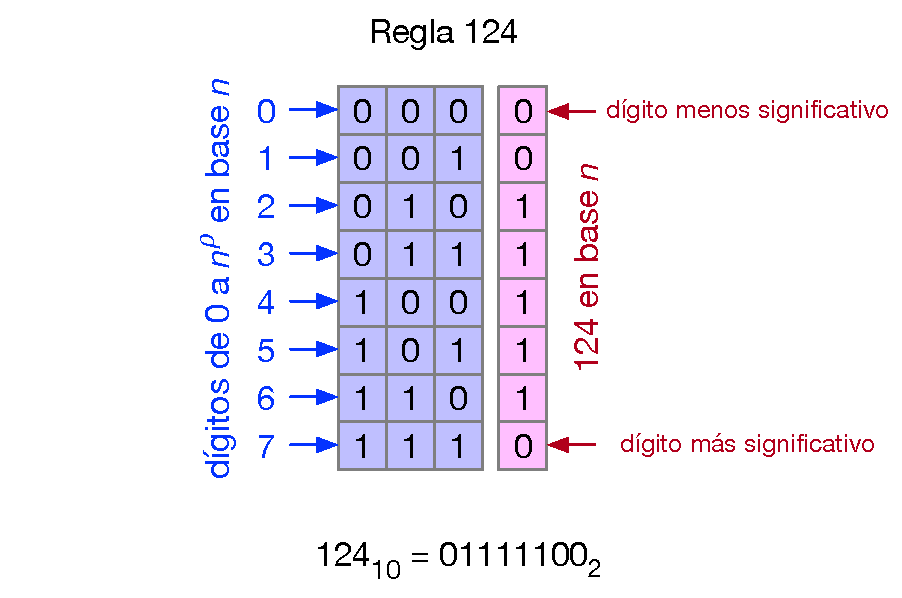
\includegraphics[width=.9\textwidth]{automata4}
\end{frame}

\begin{frame}[t]
  \frametitle{Aplicación de la regla}
  \includegraphics<+>[width=.9\textwidth]{automata51}
  \includegraphics<+>[width=.9\textwidth]{automata52}
  \includegraphics<+>[width=.9\textwidth]{automata53}
  \includegraphics<+>[width=.9\textwidth]{automata54}
  \includegraphics<+>[width=.9\textwidth]{automata55}
  \includegraphics<+>[width=.9\textwidth]{automata56}
  \includegraphics<+>[width=.9\textwidth]{automata57}
  \includegraphics<+>[width=.9\textwidth]{automata58}
  \includegraphics<+>[width=.9\textwidth]{automata59}
  \only<+>{?`cómo quedan las demás?, ?`cómo funciona la condición de frontera cíclica?}
\end{frame}

\begin{frame}[t]
  \frametitle{Ejemplos (Programa ``Autómatas Celulares'')}
  \begin{center}
  \only<+> {Regla 90, $E_{0}$=``central'' }
  \only<+> {Regla 94, $E_{0}$=``01110000000000001111100001111'' }
  \only<+> {Regla 135, $E_{0}$=``azar'' }
  \end{center}
  \begin{center}
  \includegraphics<1>[height=.6\textheight]{ac11}
  \includegraphics<2>[height=.6\textheight]{ac12}
  \includegraphics<3>[height=.6\textheight]{ac13}
  \end{center}
\end{frame}

\begin{frame}[t]
\frametitle{Clasificación de Wolfram}
\begin{itemize}[<+-| alert@+>]
	\item Uniforme
	\item Cíclico
	\item Aleatorio
	\item Complejo
\end{itemize}
\end{frame}

\begin{frame}[t]
\frametitle{Autómatas en 2D: Regla de la mayoría}
\begin{itemize}[<+->]
	\item La vida o muerte de la celda central está dictada por el valor de la mayoría de las celdas de su vecindad de Moore
\end{itemize}
\begin{center}
	\includegraphics<1>[width=.3\textwidth]{moore}
	\only<2> {Programa ``Manchas''}
	
	\includegraphics<2>[width=.5\textwidth]{manchas}
\end{center}
\end{frame}

\begin{frame}[t]
  \frametitle{Autómatas en 2D: El juego de la vida}
  \begin{itemize}[<+->]
  \item {El conjunto de símbolos es $\sigma=\{0,1\}$, significando 0=``muerta'', 1=``viva''}
  \item {$E_{0}$, y todos los demás estados, están dispuestos en una parrilla 2D de celdas}
  \item {La vecindad mide $\rho=(3,3)$, es un cuadro de $3\times 3$ símbolos}
  \item {La regla de evolución para el siguiente estado, asigna a la celda central el valor:}
  \begin{itemize}[<+->]
  \item ``viva'', si la celda central esta ``muerta'' y hay exactamente 3 vecinos vivos
  \item ``muerta'', si la celda central está ``viva'' y más de 3 (sobrepoblación) o menos de 2 (soledad) vecinos están vivos
  \item En cualquier otro caso, la celda mantiene su símbolo
  \end{itemize}
  \end{itemize}
  \begin{center}\includegraphics<+>[width=.6\textwidth]{vida1}\end{center}
\end{frame}

\begin{frame}[t]
\frametitle{Autómatas en 2D: Patrones de Turing}
\begin{columns}[t]
	\column{.7\textwidth}
	\begin{itemize}[<+->]
	\item Dos regiones elípticas, concéntricas a la celda central, cuya vida determinan
	\item Las celdas vivas en la elipse interna constituyen los activadores ($A$)
	\item Las celdas fuera de la elipse interna pero dentro de la externa constituyen los inhibidores ($I$)
	\item Hay un factor $w$ que dice que tan potentes son los inhibidores respecto a los activadores ($w=2$, significa que son el doble de potentes)
	\item Calcular $F = A - w * I$
	\begin{itemize}[<+->]
		\item Si $F >0$, la celda central vive
		\item Si $F<0$, la celda central muere
		\item Si $F=0$,  la celda central no cambia su valor
	\end{itemize}
	\end{itemize}
	\column{.3\textwidth}
	\begin{center}
		\includegraphics<1->[width=.9\textwidth]{fur1}
	\end{center}
\end{columns}
\end{frame}

\begin{frame}[t]
\frametitle{Autómatas en 2D: Patrones de Turing}
\begin{center}
	Programa ``Fur'' (biblioteca de modelos de Netlogo)
	
	\includegraphics<+>[width=.6\textwidth]{fur2}
\end{center}
\end{frame}

\begin{frame}[t]
\frametitle{Autómatas en 2D: Patrones de Turing: Observaciones}
\begin{itemize}[<+->]
	\item Nota como para ciertos valores de los parámetros, se observa la formación de patrones de ``manchas'', los cuales no dependen directamente de las reglas o el estado inicial de las celdas.
	\item Nota como en cierto momento estas ``manchas'', se estabilizan en cierta forma. Aunque algunas manchas, o fronteras de las mismas, podrían no llegar a estabilizarse.
	\item Nota también que esto aún puede considerarse autómata celular... discute por qué.
\end{itemize}

\end{frame}


\begin{frame}[t]
\frametitle{Percolación: definición}
\begin{itemize}[<+->]
	\item Se le llama percolación al traslado de alguna substancia a través de un medio ``poroso''. La substancia avanza siguiendo posiciones adyacentes de dicho medio.
	\item Ejemplos de esto son: en la ``cafetera de gotitas'', el café que atraviesa el filtro se dice que ha percolado. El petróleo u otros líquidos que se extraen de la tierra, pueden percolar a través de arena o rocas.
	\item Es relativamente sencilla su modelación mediante autómatas celulares...
	\item Ver programas ``Fire'' y ``Percolation'', en Netlogo.
\end{itemize}
\end{frame}

\begin{frame}[t]
\frametitle{Percolación: modelo}
\begin{itemize}[<+-| alert@+>]
	\item Una celda puede tener uno de tres estados: ``desocupada'', ``ocupada'' o ``utilizada''.
	\item El espacio disponible (rectángulo de celdas) se marcan unas celdas como desocupadas y otras como ocupadas, dependiendo de un valor llamado la ``densidad''.
	\item Luego de esto, en el llamado 1er estado, se marcan como ``utilizadas'', las celdas ocupadas de la columna más a la izquierda\footnote{percolación hacia la derecha, o el renglón de celdas ocupadas de más arriba, para percolar hacia abajo}.
	\item En el siguiente estado, se marcan como ``utilizadas'', las celdas del siguiente renglón que estén ocupadas y sean adyacentes\footnote{dentro de una vecindad de Moore, por ejemplo} a celdas utilizadas del estado anterior. Y así sucesivamente.
	\item Se dice que ``percola'' si al menos una celda de la columna de la derecha se torna ``utilizada''.
\end{itemize}
\end{frame}

\begin{frame}[t]
\frametitle{Percolación: variantes}
\begin{itemize}[<+->]
	\item Los modelos de Netlogo presentan unas variantes a esta definición
	\item En ``fire'', toda celda utilizada ``contagia'' a sus vecinas ocupadas, que pueden estar en columnas anteriores o siguientes.
	\item En ``percolation'', no hay celdas desocupadas, pero una utilizada ``contagia'' (o no) a cada una de sus dos vecinas del siguiente renglón, con cierta probabilidad, llamada ``porosidad''.
\end{itemize}

\end{frame}


\begin{frame}[t]
\frametitle{Percolación: ejemplos}
\begin{center}
\includegraphics<+>[height=.8\textheight]{fire}
\includegraphics<+>[height=.8\textheight]{percolation}
\end{center}
\end{frame}


\begin{frame}[t]
\frametitle{Percolación: obaservaciones}
\begin{itemize}[<+-| alert@+>]
	\item Variando la densidad, pudiera no ``percolar''. Dicho de otra forma, habrá un estado en que no haya suficientes celdas ocupadas adyacentes, a celdas utilizadas en el estado anterior.
	\item Se puede localizar el punto exacto\footnote{en realidad, como interviene el azar, esto depende de la precisión} de densidad en que ya se logra percolar\footnote{de nuevo, como interviene el azar, hay que realizar varios experimentos con la misma densidad, para ver si se obtiene el mismo resultado}.
	\item Observa que con densidad cero, no percola, y con densidad uno, si. Por lo que es posible encontrar el ``punto a partir del cual, el comportamiento cualitativo del sistema cambia''.
	\item Nota también que esto aún puede considerarse autómata celular... discute por qué.
\end{itemize}
\end{frame}

\section{Modelos Basados en Agentes}
\frame{\alert{Modelos Basados en Agentes}}

\subsection{Agentes}
\begin{frame}[t]
\frametitle{Agentes}
\begin{itemize}[<+-| alert@+>]
	\item Agente: elemento individual autónomo de una simulación computacional
	\item Tiene:
	\begin{itemize}[<+-| alert@+>]
		\item Movimiento dentro de un ambiente (``mundo'' en Netlogo)
		\item Características como memoria (variables)
		\item La autonomía de acción (funciones) que se le dé
		\item Capacidad de interactuar con su ambiente y otros agentes
		\item Los estados son menos claros, pero puede inspeccionarse el estado del sistema en un momento dado
	\end{itemize}
	\item En general tienen menos restricciones que los autómatas
	\item ?`Un agente generaliza los autómatas? o ?`todo se puede modelar con autómatas?
\end{itemize}
\end{frame}

\subsection{Introducción a Netlogo}
\begin{frame}[t]
\frametitle{Introducción a Netlogo}
\begin{itemize}[<+-| alert@+>]
	\item Lenguaje para Sistemas Complejos desarrollado por Uri Wilensky
	\item Puede verse como una generalización del lenguaje ``Logo'' (inicialmente desarrollado en el MIT)
	\item Permite manejar ``agentes'', que son principalmente las ``tortugas'' (que pueden adquirir personalidades), parches (estáticos, pero fuera de eso, son agentes también), y ``ligas'' (aristas entre tortugas, que permiten identificar las relacionadas, de ser necesario)
	\item Para programas chicos y medianos, su programación es bastante sencilla, para programas grandes, lo mejor es buscar otro lenguaje más avanzado (Python, Java, C, C++)
\end{itemize}

\end{frame}

\subsection{Elementos de Netlogo}
\begin{frame}[t]
\frametitle{Elementos de Netlogo}
\begin{itemize}[<+-| alert@+>]
	\item Pestaña ``Ejecutar''
	\begin{itemize}[<+->]
	\item ``Añadir'' (``Botón'', ``Deslizador'', ``Interruptor'', ``Seleccionador'', ``Entrada'', ``Monitor'', ``Gráfico'', ``Salida'', ``Nota'')
	\item Velocidad
	\item ticks
	\item Actualizar de la Vista (``continuamente'', ``manualmente - ticks'')
	\item Configuración
	\item Mundo
	\item Terminal de Instrucciones, Borrar, observador>
	\end{itemize}
	\item Pestaña ``Información'' (Documentación del programa)
	\item Pestaña ``Código'' (Buscar, Comprobar, Procedimientos, Sangrado automático)
	\item Menús
\end{itemize}
\end{frame}

\subsection{Mundo}
\begin{frame}[t]
\frametitle{Mundo}
\begin{itemize}[<+-| alert@+>]
	\item Es el ambiente donde se mueven los agentes
	\item Está compuesto de cuadritos contiguos llamados ``parcelas'' o ``parches''
	\item Consiste de agentes estáticos, ?`generalización de autómatas?
	\item Cada parche tiene coordenadas (enteras para su centro)
	\item En ``configuración'' (o ``editar'' con el botón derecho) se pueden modificar sus dimensiones, tamaño de parches, inicio y dirección de coordenadas, condiciones de frontera, etc.
	\item Se puede desplazar con el ratón, pero es único.
	\item El origen de sus coordenadas, el parche $(0,0)$, está en el centro.
	\item Las coordenadas $x$ y $y$ crecen hacia la derecha y hacia arriba, y decrecen en los otros sentidos.
\end{itemize}
\end{frame}


\subsection{Programas iniciales}
\begin{frame}[fragile]
\frametitle{Programas (códigos) iniciales}
\begin{itemize}[<+->]
	\item Por lo general en la ventana de código se agregan dos procedimientos: ``setup'' y ``go''
	\item ``setup'' ajusta las condiciones iniciales para el mundo y demás agentes
	\item ``go'' pone en marcha cualquier proceso que requiera la simulación
	\item Además de esto se suelen agregar deslizadores o cuadros de entrada para introducir o modificar los parámetros de la simulación
	\item El código mínimo para el setup es el siguiente:
\begin{Verbatim}[commandchars=\\\{\}]
\color{orange}to setup
    {\color{blue}clear-all}  ; se abrevia: ca
    ; agrega aquí inicialización de variables,
    ;  creación de tortugas, etc.
    ; nota los espacios a la izq. de estas líneas
    ;  indicando que están ''dentro'' de setup
    {\color{blue}reset-ticks}  ; inicializa el contador de pasos (ticks)
\color{orange}end
\end{Verbatim}
\end{itemize}
\end{frame}

\begin{frame}[t]
\frametitle{Programas iniciales}
\begin{itemize}[<+-| alert@+>]
	\item Luego de teclear este código, hay que hacer que se ejecute, por ejemplo con un botón cuyo único contenido es la llamada a la función ``setup'':
	\begin{center}{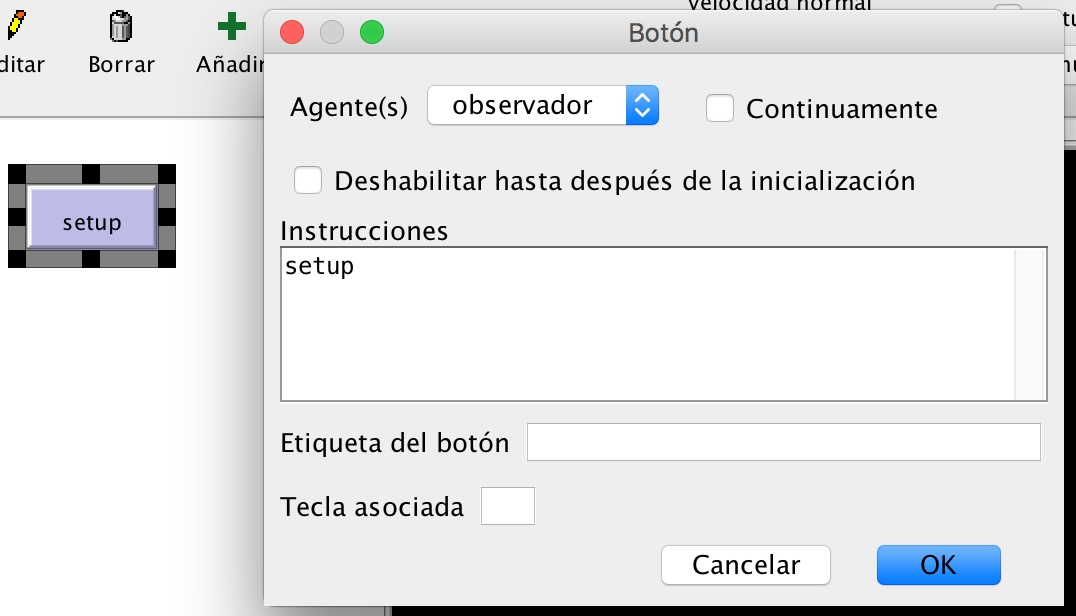
\includegraphics[width=.5\textwidth]{setup}}\end{center}
	\item Para agregar botones basta seleccionar ``Botón'' en el menú, presionar ``Añadir'' y dar click en alguna parte blanca junto al área del mundo (el ``mundo'' es el rectángulo negro de la pestaña ``Ejecutar'').
\end{itemize}
\end{frame}

\newcommand{\cb}{\color{blue}}
\newcommand{\cc}{\color{cyan}}
\newcommand{\cm}{\color{magenta}}
\newcommand{\cj}{\color{red}}

\subsection{Píntalo de rojo}
\begin{frame}[fragile]
\frametitle{Píntalo de rojo}
\begin{itemize}[<+->]
	\item Para que todos los parches realicen un mismo conjunto de acciones, utilizamos ``ask'': (después de teclear este código, agrega los botones necesarios)
	\begin{Verbatim}[commandchars=\\\{\}]
{\cc to} setup
  \cb ca
  \cb reset-ticks
\cc end

{\cc to} go
  {\cb ask} {\cm patches} [
    {\cb set} {\cm pcolor} \cj red
  ]
\cc end
\end{Verbatim}
\item ?`Qué pasa cuando presionas ``go'', pero antes haces que se ejecute ``mas lento''?, ?`Siempre es igual?
\end{itemize}
\end{frame}

\subsection{Tortugas borrachas}
\begin{frame}[t]
\frametitle{Tortugas borrachas}
\begin{itemize}[<+-| alert@+>]
	\item Veamos la creación y movimiento de tortugas
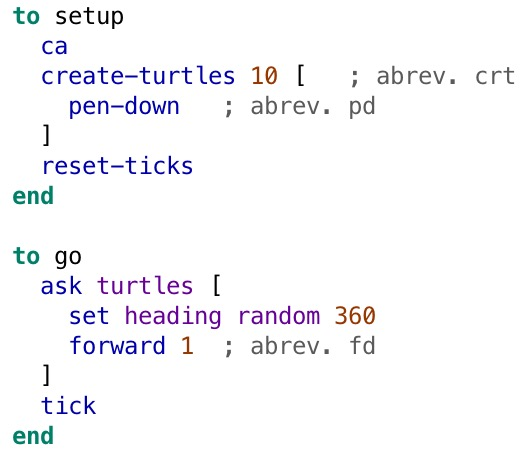
\includegraphics[width=.5\textwidth]{tortugas_borrachas}
\item Esto se puede leer: ``crea 10 tortugas, cada una: baja su pluma'', ``pídele a las tortugas: que apunten a un ángulo al azar en [0, 360); que avancen un paso'', al terminar con las tortugas: ``avanza el reloj''
\end{itemize}
\end{frame}

\begin{frame}[t]
\frametitle{Tortugas borrachas}
\begin{itemize}[<+-| alert@+>]
	\item Cada tortuga es un caminante al azar 2D. Haz las siguiente prueba:
	\item Cambia el tamaño y forma del mundo: 200x200, parcela de 1 pixel
	\item Aumenta la cantidad de tortugas a 10000
	\item Quítale el pen-down y haz que todas sean blancas
	\item Modifica el botón ``go'' para que trabaje ``continuamente''
	\item Cambia el menú de actualización a ``manualmente (ticks)''
	\item ?`Qué otra forma se te ocurre de generar caminantes al azar 2D?
\end{itemize}
\end{frame}

\subsection{Confeti}
\begin{frame}[t]
\frametitle{Confeti}
\begin{itemize}[<+-| alert@+>]
	\item Ilustra: Movimiento de agentes
\end{itemize}

\end{frame}

\subsection{Pelotas}
\begin{frame}[t]
\frametitle{Pelotas}
\begin{itemize}[<+-| alert@+>]
	\item Ilustra: Interacción de los agentes y el medio
	\item Condiciones de frontera
\end{itemize}
\end{frame}

\subsection{presaDepredador}
\begin{frame}[t]
\frametitle{presaDepredador}
\begin{itemize}[<+-| alert@+>]
	\item Ilustra: interacción de agentes entre si
	\item Presas: Deambulan aleatoriamente, cada cierto tiempo se reproducen
	\item Depredador: Al encontrar una presa cerca, se la come. Luego de cierto tiempo de no comer, muere. Luego de cierto tiempo, se reproduce.
	\item comportamiento complejo?
\end{itemize}
\end{frame}

\subsection{rapidosVSlentos}
\begin{frame}[t]
\frametitle{rapidosVSlentos}
\begin{itemize}[<+-| alert@+>]
	\item Ilustra: interacción de agentes con medio
	\item Interacción de agentes entre si
	\item discutir: emergencia de comportamiento complejo?
\end{itemize}
\end{frame}

\begin{frame}[t]
\frametitle{Segregación}
\begin{itemize}[<+-| alert@+>]
	\item Esta versión del modelo inicialmente propuesto por Thomas Schelling, simula las interacciones y bloques de comunidades que se segregan (viven junto a los ``suyos'')
	\item Cada agente que tiene al menos un cierto porcentaje de vecinos de su mismo color (que representa alguna preferencia), se siente ``feliz''.
	\item Los agentes infelices buscan situarse en alguna otra celda desocupada.
	\item Con el tiempo los agentes se ponen más felices, pero la vecinadad se hace más segregada
	\item Basta desear un 30\% de vecinos del mismo color para que acaben con un promedio de 70\% de vecinos del mismo color
\end{itemize}

\end{frame}


\subsection{El Farol}
\begin{frame}[t]
\frametitle{El Farol (cap. 3 Uri)}
\begin{itemize}[<+-| alert@+>]
	\item Las noches del jueves, en el bar ``El Farol'' de Santa Fe se puede escuchar música irlandesa.
	\item Pero a veces se llena, y si los clientes piensan que así será, se quedan en casa.
	\item El modelo entonces representa la asistencia de clientes al bar, siguiendo algunas estrategias. Cada una ayuda al cliente a decidir si asistirá o no esta semana, basándose en que tan lleno estuvo el bar semanas antes (MEMORY-SIZE).
	\item La mejor estrategia para un cliente sería siempre asistir, ya que no se lo penaliza si el bar se llena. Sin embargo no se trata de optimizar la asistencia si no está lleno, sino el predecir cuando asistir y ver como se comporta el grupo.
	\item Los clientes usan alguna de NUMBER-STRATEGIES estrategias para decidir asistir o no esta semana, y aunque inicialmente se les asigna la estrategia al azar, este las va puntuando dependiendo de que tan buena le resultó.
\end{itemize}

\end{frame}


\end{document}